%% abtex2-modelo-trabalho-academico.tex, v-1.9.6 laurocesar
%% Copyright 2012-2016 by abnTeX2 group at http://www.abntex.net.br/ 
%%
%% This work may be distributed and/or modified under the
%% conditions of the LaTeX Project Public License, either version 1.3
%% of this license or (at your option) any later version.
%% The latest version of this license is in
%%   http://www.latex-project.org/lppl.txt
%% and version 1.3 or later is part of all distributions of LaTeX
%% version 2005/12/01 or later.
%%
%% This work has the LPPL maintenance status `maintained'.
%% 
%% The Current Maintainer of this work is the abnTeX2 team, led
%% by Lauro César Araujo. Further information are available on 
%% http://www.abntex.net.br/
%%
%% This work consists of the files abntex2-modelo-trabalho-academico.tex,
%% abntex2-modelo-include-comandos and abntex2-modelo-references.bib
%%
%% ------------------------------------------------
%% Este arquivo é baseado na classe abnTeX2 e foi editado por Guilherme Boaviagem Ribeiro (guilherme.boaviagem@gmail.com) visando
%% se adequar às normas da Biblioteca do Centro de Tecnologia e Geociências (CTG) da Universidade
%% Federal de Pernambuco (UFPE). Em março de 2018 este layout foi aceito na Biblioteca Central,
%% como parte dos protocolos após a defesa.
% % ------------------------------------------------


% ------------------------------------------------------------------------
% ------------------------------------------------------------------------
% abnTeX2: Modelo de Trabalho Academico (tese de doutorado, dissertacao de
% mestrado e trabalhos monograficos em geral) em conformidade com 
% ABNT NBR 14724:2011: Informacao e documentacao - Trabalhos academicos -
% Apresentacao
% ------------------------------------------------------------------------
% -----------------------------------------------------------------------
%==============================================
\documentclass[
	% -- opções da classe memoir --
	12pt,				% tamanho da fonte
	openright,			% capítulos começam em pág ímpar (insere página vazia caso preciso)
	oneside,			% para impressão em recto e verso. Oposto a oneside
	a4paper,			% tamanho do papel. 
	fleqn,              % Neto - Tentando alinhar todas as equacoes
	% -- opções da classe abntex2 --
	chapter=TITLE,		% títulos de capítulos convertidos em letras maiúsculas
	section,		% títulos de seções convertidos em letras maiúsculas
	%subsection=TITLE,	% títulos de subseções convertidos em letras maiúsculas
	%subsubsection=TITLE,% títulos de subsubseções convertidos em letras maiúsculas
	sumario=abnt-6027-2012,
	% -- opções do pacote babel --
	english,			% idioma adicional para hifenização
	french,				% idioma adicional para hifenização
	spanish,			% idioma adicional para hifenização
	brazil				% o último idioma é o principal do documento
	]{abntex2}
%==============================================-
\makeatletter
  \@ifclasswith{abntex2}{chapter=TITLE}{
    \begingroup
    \def\x#1chapter=TITLE,#2\@nil{%
      \endgroup\def\@classoptionslist{#1#2}%
    }\expandafter\x\@classoptionslist\@nil
  }{}

  \@ifclasswith{abntex2}{section=TITLE}{
    \begingroup
    \def\x#1section=TITLE,#2\@nil{%
      \endgroup\def\@classoptionslist{#1#2}%
    }\expandafter\x\@classoptionslist\@nil
  }
\makeatother
%==============================================-

% Pacotes básicos
% ---
%\usepackage{lmodern}			% Usa a fonte Latin Modern(lmodern)	% arev -> Parece com Arial
\usepackage{times}					 			%%%
%\renewcommand{\familydefault}{\sfdefault}		%%%
\usepackage[T1]{fontenc}		% Selecao de codigos de fonte.
\usepackage[utf8]{inputenc}		% Codificacao do documento (conversão automática dos acentos)
\usepackage{lastpage}			% Usado pela Ficha catalográfica
\usepackage{indentfirst}		% Indenta o primeiro parágrafo de cada seção.
\usepackage{color}				% Controle das cores
\usepackage{graphicx}			% Inclusão de gráficos
\usepackage{subfig}				% Inclusão de Subfiguras
\usepackage{microtype} 			% para melhorias de justificação
\usepackage{pdfpages}           % insere páginas PDF
\usepackage{nomencl}			% insere nomenclatura
\usepackage{multirow}
\usepackage{calc}
\usepackage{mathtools}
\usepackage{cite}
\usepackage{amsmath}
\usepackage{siunitx}
\usepackage{lipsum}
\usepackage{minted}
\usepackage{float}

\usepackage{colortbl}
\usepackage{makecell}
\usepackage[dvipsnames]{xcolor}


% Pacotes adicionados por mim (Jose Rodrigues de Oliveira Neto)
%\usepackage{indentfirst}
\usepackage{lettrine}
\usepackage{amsmath,amsfonts,amsthm}										% Math packages
\usepackage{epsfig,subfig}
\usepackage{mathdots,multirow,tabu}
%\usepackage[pdftex]{graphicx}											% Enable pdflatex
\usepackage{url}
\usepackage{etoolbox}
\gappto{\UrlBreaks}{\UrlOrds}
\usepackage{enumerate}
\usepackage{color}
\usepackage{rotating}           % rotacionar tabelas
% ---
% ---
\usepackage{amssymb}     % qed
\usepackage{thmtools}    % Front end para amsthm (\declaretheorem)
\declaretheorem[style=definition,name=Definição,parent=chapter,qed=]{definition} %\qedsymbol
\declaretheorem[style=plain,name=Lema,parent=chapter,qed=]{lemma}
\declaretheorem[style=plain,name=Teorema,parent=chapter,qed=]{theorem}
\declaretheorem[style=plain,name=Axioma,parent=chapter,qed=]{axioma}
\declaretheorem[style=plain,name=Corolário,parent=chapter,qed=]{corollary}
\declaretheorem[style=plain,name=Proposição,parent=chapter,qed=]{proposition}
\declaretheorem[style=plain,name=Prova,numbered=no,qed=$\blacksquare$]{prova}
\declaretheorem[style=plain,name=Propriedade,parent=chapter,qed=]{property}

\newcommand{\bfemph}[1]{\textbf{#1}} %Mudar o emph de itálico para negrito para tentar resolver o problema das citações que mudou na nova NBR 6023-2018
\renewcommand{\emph}[1]{\bfemph{#1}}

%\setlength{\mathindent}{0pt} %Tentando alinha todas as equações
% FIM (Jose Rodrigues de Oliveira Neto)

% ---
\renewcommand{\ABNTEXchapterfont}{\fontfamily{cmr}\fontseries{b}\selectfont}
\usepackage[brazilian,hyperpageref]{backref}	 % Paginas com as citações na bibl
\usepackage[alf]{abntex2cite}	% Citações padrão ABNT


% NEW COMMANDS
\newcommand{\doublecitep}[2]{\citep[como citado em \citealp{#2}]{#1}} % double citations, the result is \citep[como citado em  \citealp{someotherguykey2013}]{someguykey2010}

\renewcommand{\ABNTEXsubsubsectionfont}{\rmfamily\mdseries}
\renewcommand{\ABNTEXsubsubsectionfontsize}{\normalsize}

\renewcommand{\ABNTEXsubsectionfont}{\rmfamily\mdseries}
\renewcommand{\ABNTEXsubsectionfontsize}{\normalsize}

\renewcommand{\ABNTEXsectionfont}{\rmfamily\bfseries}
\renewcommand{\ABNTEXsectionfontsize}{\normalsize}

\renewcommand{\ABNTEXchapterfont}{\ABNTEXsectionfont\bfseries}
\renewcommand{\ABNTEXchapterfontsize}{\normalsize}
%
% Fontes das entradas do sumario
%
\renewcommand{\cftsubsubsectionfont}{\mdseries} 
\renewcommand{\cftsubsubsectionpagefont}{\cftsubsectionfont}

\renewcommand{\cftsubsectionfont}{\mdseries} 
\renewcommand{\cftsubsectionpagefont}{\cftsubsectionfont}
%
\renewcommand{\cftsectionfont}{\bfseries}
\renewcommand{\cftsectionpagefont}{\cftsectionfont}
%
\renewcommand{\cftchapterfont}{\bfseries}
\renewcommand{\cftchapterpagefont}{\normalsize\cftchapterfont}

\renewcommand{\folhaderostoname}{FOLHA DE ROSTO}
\renewcommand{\epigraphname}{EP\'IGRAFE}
\renewcommand{\dedicatorianame}{DEDICAT\'ORIA}
\renewcommand{\agradecimentosname}{AGRADECIMENTOS}
\renewcommand{\folhadeaprovacaoname}{FOLHA DE APROVA\c C\~AO}
\renewcommand{\resumoname}{RESUMO}
\renewcommand{\listadesimbolosname}{LISTA DE S\'IMBOLOS}
\addto\captionsbrazil{% portugues-brasil
	%% ajusta nomes padroes do babel
	\renewcommand{\bibname}{REFER\^ENCIAS}
	\renewcommand{\listfigurename}{LISTA DE ILUSTRA\c C\~OES}
	\renewcommand{\listtablename}{LISTA DE TABELAS}
	\renewcommand{\contentsname}{SUM\'ARIO}
	%% ajusta nomes usados com a macro \autoref
}





\makeatother

% --- 
% CONFIGURAÇÕES DE PACOTES
% --- 

% ---
% Configurações do pacote backref
% Usado sem a opção hyperpageref de backref
\renewcommand{\backrefpagesname}{Citado na(s) página(s):~}
% Texto padrão antes do número das páginas
\renewcommand{\backref}{}
% Define os textos da citação
\renewcommand*{\backrefalt}[4]{
	\ifcase #1 %
		Nenhuma citação no texto.%
	\or
		Citado na página #2.%
	\else
		Citado #1 vezes nas páginas #2.%
	\fi}%
% ---




% ---
% Configurações de aparência do PDF final

% alterando o aspecto da cor azul
\definecolor{blue}{RGB}{41,5,195}

% informações do PDF
\makeatletter
\hypersetup{
     	%pagebackref=true,
		pdftitle={\@title}, 
		pdfauthor={\@author},
    	pdfsubject={\imprimirpreambulo},
	    pdfcreator={LaTeX with abnTeX2},
		pdfkeywords={abnt}{latex}{abntex}{abntex2}{trabalho acadêmico}, 
		colorlinks=true,       		% false: boxed links; true: colored links #aqui
    	linkcolor=black,          	% color of internal links
    	citecolor=black,        		% color of links to bibliography
    	filecolor=black,      		% color of file links
		urlcolor=blue,
		bookmarksdepth=4
}
\makeatother
% --- 

% --- 
% Espaçamentos entre linhas e parágrafos 
% --- 

% O tamanho do parágrafo é dado por:
\setlength{\parindent}{1.3cm}

% Controle do espaçamento entre um parágrafo e outro:
\setlength{\parskip}{0.2cm}  % tente também \onelineskip

% ---
% compila o indice
% ---
\makeindex
% ---

% ----
% Início do documento
% ----
\begin{document}

% Seleciona o idioma do documento (conforme pacotes do babel)
%\selectlanguage{english}
\selectlanguage{brazil}

% Retira espaço extra obsoleto entre as frases.
\frenchspacing 

% ----------------------------------------------------------
% ELEMENTOS PRÉ-TEXTUAIS
% ----------------------------------------------------------
% \pretextual

% ---
% Capa
% ---
% ---
% Informações de dados para CAPA e FOLHA DE ROSTO
% ---
% ---
% Informações de dados para CAPA e FOLHA DE ROSTO
% ---Construção de Autovetores de Transformadas Discretas de Fourier: Novos Métodos e Aplicações
\titulo{\uppercase{RELAT\'ORIO DA PRIMEIRA PR\'ATICA DE ELETR\^ONICA DIGITAL }
\textnormal{}}
\autor{\uppercase{GABRIELA LEITE PEREIRA\\BRUNO FRANCA GUIMAR\~AES\\PEDRO LUCAS DE SOUZA LE\~AO\\HENRIQUE PEDRO DA SILVA}}
\local{\uppercase{Recife}}
\data{2023}
%\orientador{Dr. Marco Aurélio Benedetti Rodrigues}
%\coorientador{} % Comentar aqui, caso apropriado.
\instituicao{%
  UNIVERSIDADE FEDERAL DE PERNAMBUCO
  \\ %\par
  CENTRO DE TECNOLOGIA E GEOCIÊNCIAS
  \\ %\par
  DEPARTAMENTO DE ELETRÔNICA E SISTEMAS
  \\ %\par 
  PROGRAMA DE P\'OS-GRADUA\c C\~AO EM ENGENHARIA EL\'ETRICA
  }
\tipotrabalho{Tese (Doutorado)}

\preambulo{
\uppercase{INFORMA\c C\~OES DA DISCIPLINA}\\
Curso : ENGENHARIA ELETRÔNICA – CTG\\
Disciplina: ELETRÔNICA DIGITAL 1A\\
Código: ES441, Turma: EB, Semestre: 2021.2\\
\\
DOCENTE RESPONSÁVEL: DR. MARCO AURÉLIO BENEDETTI RODRIGUES\\
DOCENTE ESTAGIÁRIO: MSC. MALKI-ÇEDHEQ B. C. SILVA
}
% ---
\imprimircapa
% ---

% ---
% Folha de rosto
% (o * indica que haverá a ficha bibliográfica)
% ---
\imprimirfolhaderosto*
% ---

% ---
% Inserir a ficha catalográfica
% ---

% Isto é um exemplo de Ficha Catalográfica, ou ``Dados internacionais de
% catalogação-na-publicação''. Você pode utilizar este modelo como referência. 
% Porém, provavelmente a biblioteca da sua universidade lhe fornecerá um PDF
% com a ficha catalográfica definitiva após a defesa do trabalho. Quando estiver
% com o documento, salve-o como PDF no diretório do seu projeto e substitua todo
% o conteúdo de implementação deste arquivo pelo comando abaixo:
%
%\begin{fichacatalografica} %Descomentar caso necessário 
%\includepdf{DECLARACOES/fichacatalografica.pdf}
%\end{fichacatalografica}

%\begin{fichacatalografica} %Descomentar caso necessário 
%\includepdf{DECLARACOES/Ata_Sidney_assinado_HAC_assinado.pdf}
%\end{fichacatalografica}

%\begin{fichacatalografica}
%\vspace*{\fill}
%	\sffamily
%	\vspace*{\fill}					% Posição vertical
%	\begin{center}					% Minipage Centralizado
%	\fbox{\begin{minipage}[c][8cm]{13.5cm}		% Largura
%	\small
%	\imprimirautor
%	%Sobrenome, Nome do autor
%	
%	\hspace{0.5cm} \imprimirtitulo  / \imprimirautor. --
%	\imprimirlocal, \imprimirdata-
%	
%	\hspace{0.5cm} \pageref{LastPage} p. : il. (algumas color.) ; 30 cm.\\
%	
%	\hspace{0.5cm} \imprimirorientadorRotulo~\imprimirorientador\\
%	
%	\hspace{0.5cm}
%	\parbox[t]{\textwidth}{\imprimirtipotrabalho~--~\imprimirinstituicao,
%	\imprimirdata.}\\
%	
%	\hspace{0.5cm}
%		1. Palavra-chave1.
%		2. Palavra-chave2.
%		2. Palavra-chave3.
%		I. Orientador.
%		II. Universidade xxx.
%		III. Faculdade de xxx.
%		IV. Título 			
%	\end{minipage}}
%	\end{center}

%\end{fichacatalografica}
% ---

% ---
% Inserir errata
% ---
%\begin{errata}
%Elemento opcional da \citeonline[4.2.1.2]{NBR14724:2011}. Exemplo:
%
%\vspace{\onelineskip}
%
%FERRIGNO, C. R. A. \textbf{Tratamento de neoplasias ósseas apendiculares com
%reimplantação de enxerto ósseo autólogo autoclavado associado ao plasma
%rico em plaquetas}: estudo crítico na cirurgia de preservação de membro em
%cães. 2011. 128 f. Tese (Livre-Docência) - Faculdade de Medicina Veterinária e
%Zootecnia, Universidade de São Paulo, São Paulo, 2011.
%
%\begin{table}[htb]
%\center
%\footnotesize
%\begin{tabular}{|p{1.4cm}|p{1cm}|p{3cm}|p{3cm}|}
%  \hline
%   \textbf{Folha} & \textbf{Linha}  & \textbf{Onde se lê}  & \textbf{Leia-se}  \\
%    \hline
%    1 & 10 & auto-conclavo & autoconclavo\\
%   \hline
%\end{tabular}
%\end{table}
%
%\end{errata}
% ---

% ---
% Inserir folha de aprovação
% ---

% Isto é um exemplo de Folha de aprovação, elemento obrigatório da NBR
% 14724/2011 (seção 4.2.1.3). Você pode utilizar este modelo até a aprovação
% do trabalho. Após isso, substitua todo o conteúdo deste arquivo por uma
% imagem da página assinada pela banca com o comando abaixo:
%
%\includepdf{folhadeaprovacao.pdf}
% DESCOMENTAR CASO NECESSÁRIO
%\begin{folhadeaprovacao}
%
%\begin{center}
%
%{\rmfamily\mdseries\normalsize\imprimirautor}
%\vspace*{\fill}\vspace*{\fill}
%\begin{center}
%  \rmfamily\bfseries\normalsize\imprimirtitulo
%\end{center}
%\vspace*{\fill}
%
%\hspace{.45\textwidth}
%\begin{minipage}{.5\textwidth}
%    \imprimirpreambulo
%\end{minipage}%
%\vspace*{\fill}
%\end{center}    
%Aprovado em: $\underline{\quad 23\quad }\mathbf{/}\underline{\quad 01 \quad }/\underline{\,\,\,2019\,\,\,}$.
%\assinatura{\imprimirorientador ~(Orientador) \\ Universidade Federal de Pernambuco} 
%\assinatura{\imprimircoorientador (Coorientador) \\  Carleton University}
%\assinatura{Prof. Dr. Ricardo Menezes Campello de Souza (Examinador Interno) \\ Universidade Federal de Pernambuco}
%\assinatura{Prof. Dr. Daniel Pedro Bezerra Chaves (Examinador Interno) \\ Universidade Federal de Pernambuco}
%\assinatura{Prof. Dr. Eduardo Shirlippe Goes Leandro (Examinador Externo) \\ Universidade Federal de Pernambuco}
%\assinatura{Prof. Dr. Francisco Madeiro Bernardino Jr. (Examinador Externo) \\  Universidade de Pernambuco}
%  
%%\begin{center}
%%{\normalsize\imprimirlocal}
%%\par
%%{\normalsize\imprimirdata}
%%%\vspace*{1cm}
%%\end{center}
%
%\end{folhadeaprovacao}
% ---

% --------------------------------------
% Dedicatória
% --------------------------------------

%% ---
% Dedicatória
% ---
\begin{dedicatoria}
   \vspace*{\fill}
   \raggedright%\centering
   \noindent
   \textit{Dedico esse trabalho .....} %\vspace*{3cm}
\end{dedicatoria}
% ---

% --------------------------------------
% Epígrafe
% --------------------------------------
%% ---
% Epígrafe
% ---
\begin{epigrafe}
    \vspace*{\fill}
	\begin{flushright}
		\textit{``In literature, an epigraph is a phrase, quotation, or poem that is set at the beginning of a document or component. The epigraph may serve as a preface, as a summary, as a counter-example, or to link the work to a wider literary canon, either to invite comparison or to enlist a conventional context.'' \\
			(Nature)}
	\end{flushright}
\end{epigrafe}
% ---


% --------------------------------------
% RESUMOS
% --------------------------------------

% ---
% RESUMOS
% ---
\begin{comment}
% resumo em português
\setlength{\absparsep}{18pt} % ajusta o espaçamento dos parágrafos do resumo
\begin{resumo}

%==========================================
\hspace{1.1cm}
“Malware” é uma junção dos termos “malicioso” e “software”. O malware tem como principal objetivo acessar um dispositivo alheio sem permissão explícita de seu proprietário. 
Dentre os malwares, as Ameaças Persistentes Avançadas, do inglês \textit{Advanced Persistent Threat} (APT), ganharam muito espaço no tópico de roubo de dados e comportamento destrutivo para softwares, principalmente quando se trata de organizações federais e indústrias privadas de grande porte, devido à complexidade e eficiência desse tipo de ataque. Os malwares do tipo APT são direcionado para um alvo pré-definido sendo sempre bem orquestrado com grande precisão e controle, aproveitando os recursos de reconhecimento e vulnerabilidades avançadas.
%----------------------------------------
 O presente trabalho propõe uma análise crítica acerca do desempenho dos principais antivírus comerciais atuais quanto à detecção de malwares do tipo APT.
 Em acréscimo, são replicados antivírus do estado da arte dotados de distintas metodologias de detecção baseadas no princípio de redes neurais. 
 Como contribuição principal, um antivírus autoral é criado por meio de uma máquina de aprendizagem extrema e com kernels de processamento pseudo-morfológicos. O referido antivírus autoral tem o intuito de apresentar uma alternativa criativa, eficaz e rápida no controle desse tipo de malware. 
Por último, são apresentados os resultados da aplicação e sua comparação com os demais antivírus do estado da arte.
%----------------------------------------
O antivírus autoral alcança um desempenho médio de 93,62\% na
distinção entre aplicativos benignos e APT acompanhado de um tempo treinamento de 0,55 segundos, em média.
Espera-se que o antivírus inteligente autoral atue de forma preventiva e impeça que os malwares do tipo APT
causem prejuízos às instituições privadas e autarquias públicas. 
%----------------------------------------

\textbf{Palavras-chave}: Antivírus, Detecção de malwares, Ameaças persistentes Avançadas, Máquina de aprendizagem extrema.
\end{resumo}

% resumo em inglês
\begin{resumo}[ABSTRACT]
 \begin{otherlanguage*}{english}
\hspace{1.1cm} "Malware" is a joining of the terms "malicious" and "software." Malware is primarily intended to access another's device without the owner's explicit permission. 
Among malware, Advanced Persistent Threats (APT) have gained much ground on the topic of data theft and destructive behavior for software, especially when it comes to federal organizations and large private industries, due to the complexity and efficiency of this type of attack. APT-type malware is directed at a predefined target and is always well-orchestrated with great precision and control, taking advantage of advanced vulnerability recognition capabilities.
%----------------------------------------
 This paper proposes a critical analysis of the performance of the current main commercial antivirus products in detecting APT malware.
 In addition, state of the art antivirus programs with different detection methodologies based on the neural network principle are replicated. 
 As a main contribution, an authoral antivirus is created by means of an extreme learning machine with pseudo-morphological processing kernels. This authorial antivirus is intended to present a creative, effective and fast alternative in the control of this type of malware. 
Finally, the results of the application and its comparison with other state of the art antiviruses are presented.
%----------------------------------------
The author antivirus reaches an average performance of 93.62\% in
distinction between benign and APT applications accompanied by a training time of 0.55 seconds on average.
The intelligent authoring antivirus is expected to act preventively and stop APT malware from malware from harming private institutions and public autarchies. 

   \vspace{\onelineskip}
 
   \noindent 
   \textbf{Keywords}: Antivirus, Malware detection, Advanced persistent threats, Extreme learning machine.
 \end{otherlanguage*}
\end{resumo}

%% resumo em francês 
%\begin{resumo}[Résumé]
% \begin{otherlanguage*}{french}
%    Il s'agit d'un résumé en français.
% 
%   \textbf{Mots-clés}: latex. abntex. publication de textes.
% \end{otherlanguage*}
%\end{resumo}
%
%% resumo em espanhol
%\begin{resumo}[Resumen]
% \begin{otherlanguage*}{spanish}
%   Este es el resumen en español.
%  
%   \textbf{Palabras clave}: latex. abntex. publicación de textos.
% \end{otherlanguage*}
%\end{resumo}
% ---
\end{comment}

% --------------------------------------
% inserir lista de ilustrações
% --------------------------------------
%\pdfbookmark[0]{\listfigurename}{lof}
%\listoffigures*
%\cleardoublepage


% --------------------------------------
% inserir lista de tabelas
% --------------------------------------
%\pdfbookmark[0]{\listtablename}{lot}
%\listoftables*
%\cleardoublepage



% --------------------------------------
% inserir lista de abreviações
% --------------------------------------
% ---
% inserir lista de abreviaturas e siglas
% ---
\begin{comment}
\begin{siglas}
  \item[bpp]    Bits por pixel
  \item[DFT]    Discrete Fourier transform (Transformada de Fourier Discreta)
\item[APT]    Advanced Persistent Threat (Ameaça Persistente Avançada)
 \item[MLP]    Multilayer Perceptron (Perceptron Multicamadas)
 \item[ELM]    Extreme Learning Machine (Máquinas de aprendizado extremo)
 \item [mELMs]    Morphological Extreme Learning Machine (Máquina Morfológica de Aprendizagem Extrema)
 \item[ReLU]   Rectified Liear Unit (Unidade Linear Retificada)
 \item[LSTM]    Long Short Term Memory (memória de curto prazo longa)
 \item[RBM]    Restricted Boltzmann Machine (Máquina Boltzmann Restrita)
 \item[UC]    Unidade de Controle 
 \item[RAM]    Random Acess Memory (Memória de Acesso Aleatório)
 \item[TLS]    Transport Layer Security (Segurança da Camada de Transporte)
 \item[API]    Application Programming Interface (Interface de Programação de Aplicativos)
 \item[OS]    Operational System (Sistema Operacional)
 \item[GUI]    Graphical User Interface (Interface gráfica do usuário)
 \item[DNS]    Domain Name System (Sistema de Nomes de Domínio)
 \item[FTP]    File Transfer Protocol (Protocolo de transferência de arquivos)
 \item[HTTP]   Hypertext Transfer Protocol (Protocolo de Transferência de Hipertexto)
\end{siglas}
% ---
\end{comment}


% --------------------------------------
% inserir o sumario
% --------------------------------------
\pdfbookmark[0]{\contentsname}{toc}
\tableofcontents*
\cleardoublepage


% ----------------------------------------------------------
% ELEMENTOS TEXTUAIS
% ----------------------------------------------------------
\textual

\chapter{INTRODUÇÃO} \label{cap_1_Introducao}

Nessa primeira prática, a utilização da \emph{FPGA} foi para descobrir uma senha de 16 valores hexadecimais, que foi fixada pelo grupo. Para descobrir essa senha tem-se várias tentativas.


O objetivo do trabalho é a utilização da plataforma quartus e, por meio de portas lógicas, flip-flops e outros recursos dela em diagrama de blocos, elaborar o sistema pedido na primeira prática. Para atingir esse objetivo, é necessário: a elaboração de contadores MOD10 e MOD2, a elaboração de armazenadores de valores hexadecimais de 4 bits e conexão entre as tentativas de adivinhar a senha com certos leds e buzzer, com devidas frequências.


Este relatório estará dividido em 5 seções. A primeira é o desenvolvimento, no qual será explicado as etapas em que foi feito so processo com suas devidas explicações. A segunda é o manual de operações, no qual será explicado todo o funcionamento do hardware projetado na fpga. A terceira é os resulatdos, que terá, em ordem, o que foi obtido como resposta ao longo do desenvolvimento do projeto. A quarta é a discussão dos resultados, que abordará do porque desses resultados terem sido atingidos. A última é a conclusão que irá discutir, de forma resumida, se os resultados obtidos foram os solicitados no projeto.  



\chapter{Desenvolvimento}\label{cap_2_Fundamentaçao}

Neste capítulo, será discutido, inicialmente, uma visão geral do circuito completo e como seus componentes se comportam em conjunto para gerar um jogo de checagem de senha.

Após isso, detalhes de cada componente do circuito serão discutidos, além de como foi construído componentes maiores a partir de componentes mais basicos.

\section{O Circuito Completo}

%Estes quem?(segunda linha)
Neste circuito, visto na Figura \ref{fig:2.1}, tem-se os inputs dos botões entrando diretamente no \emph{Chave Led Buzzer}, descrito em 2.11. Estas chaves ligaram diretamente nos LEDs para indicar quais bits do hexadecimal de entrada estão ativos.

\begin{figure}[H]
	\centering
	\includegraphics[width=1\columnwidth]{FIGURAS/cap_2/projeto.png}
	\caption{Representação esquemática do projeto completo.}
        \label{fig:2.1}
\end{figure}


Estes bits serão levados até o comparador. Lá, eles serão comparados com os bits que estão saindo do banco de registrador.

Simultaneamente, tem-se um clock com frequência de $1Hz$ sendo inserido em um contador módulo 10. Sua saída será transformada em pulso. Essa transformação é feita para poder-se ter um rising edge tanto na subida, quanto na descida do clock.

Este pulso será levado de volta pros \emph{Chave Led Buzzer} para dar reset neles, e permitir ao usuário a inserção do próximo dígito.

Estes pulsos também seguiram e bifurcaram em dois caminhos, dependendo do estado atual do comparador. Se o comparador confirmar que os dígitos estão corretos com os do hexadecimal de senha atual, um clock será dado no banco de registradores para pular pro próximo dígito, e uma frequência aguda é emitida no buzzer. Essa frequência dará mute nas frequências vindas dos botões.

Se o comparador afirmar que o dígito estava errado, o banco de comparadores é resetado e retorna-se ao primeiro hexadecimal.

Caso o registrador estore sua contagem, conclui-se que o último dígito da senha foi inserido corretamente, desconecta-se o clock de entrada do contador, da-se mute em todas frequências vindas dos botões e ativa-se uma frequência aguda para confirmar que o programa foi concluído.

Todas as frequências, exceto a de finalização do programa, estão em um sistema de prioridade descrito em 2.9, para impedir interferências.



\section{Flip-Flops}

Foi utilizado dois tipos de flip-flops no projeto, o tipo \emph{t} e o tipo \emph{d}.

Ambos têm entrada clear e preset, que quando estão, ambas, em nível lógico alto (1,1), não afetam a saída Q dos flip-flops.

Quando uma delas está em nível lógico baixo e a outra em nível lógico alto, elas tomam precedência sobre as entradas do flip-flop. A saída será definida como 1 se preset estiver em nível lógico baixo, ou 0, se o clear estiver em nível lógico baixo.

É um estado proibido ambos, clear e preset, estarem em nível lógico baixo (0,0).

\subsection{Tipo \emph{t}}

Na Figura \ref{fig:2.2} pode-se observar a representação do flip-flop tipo \emph{t}.

\begin{figure}[H]
	\centering
	\includegraphics[width=0.3\columnwidth]{FIGURAS/cap_2/tff.png}
	\caption{Representação do flip-flop tipo t.}
        \label{fig:2.2}
\end{figure}

Neste flip-flop, a entrada \emph{T} define se a saída será invertida ou não quando houver uma subida (rising\_edge) do clock.

Este flip-flop foi utilizado extensivamente no modo inversor, ou seja com o \emph{T} em nível lógico alto.

\subsection{Tipo \emph{d}}

Na Figura \ref{fig:2.3} pode-se observar a representação do flip-flop tipo \emph{d}.

\begin{figure}[H]
	\centering
	\includegraphics[width=0.3\columnwidth]{FIGURAS/cap_2/dff.png}
	\caption{Representação do flip-flop tipo d.}
        \label{fig:2.3}
\end{figure}

O flip-flop \emph{d}, passa o valor da entrada para a saída quando há uma subida (rising\_edge) no nível lógico do clock.

Ele foi utilizado como buffer de informação no tipo de conexão \emph{Q->D} e como inversor (similar ao tipo \emph{t}) quando \emph{NOT Q -> D}.

\section{Divisores}

Foi criado divisores de clock para controlar as mudanças de frequência do circuito. E também para estabilizar pulsos em clocks.

\subsection{Divisor1}

Na Figura \ref{fig:2.4} é apresentado o Divisor1.

\begin{figure}[H]
	\centering
	\includegraphics[width=1\columnwidth]{FIGURAS/cap_2/divisor1.png}
	\caption{Representação do Divisor1, que divide o clock pela metade.}
        \label{fig:2.4}
\end{figure}

Ele fará uma divisão de clock, de maneira decrescente utilizando um flip-flop do tipo \emph{d} na configuração inversora.

%Essa frase ficou certa?
Foi utilizado o modo decrescente, pois este era um requerimento do projeto para o controle do tempo do buzzer.

\subsection{Divisor8}

Neste, tem-se 8 Divisor1 em série, como pode ser visto na Figura \ref{fig:2.5}. Ele foi feito para dividir o clock em $2^8$.

\begin{figure}[H]
	\centering
	\includegraphics[width=1\columnwidth]{FIGURAS/cap_2/divisor8.png}
	\caption{Representacao do Divisor8, que divide o clock por $2^8$.}
        \label{fig:2.5}
\end{figure}

Ele foi utilizado para simplificar o diagrama de blocos quando precisa-se  dividir o clock por valores grandes.



\subsection{Divisor16}

Neste, tem-se 2 Divisor8 em série, como pode ser visto na Figura \ref{fig:2.6}. Ele foi feito para dividir o clock em $2^{16}$.

\begin{figure}[H]
	\centering
	\includegraphics[width=1\columnwidth]{FIGURAS/cap_2/divisor16.png}
	\caption{Representacao do Divisor8, que divide o clock por $2^{16}$.}
        \label{fig:2.6}
\end{figure}


Ele também foi utilizdo para simplificar o diagrama de blocos quando precisa-se dividir o clock por valores grandes.



\section{Contadores}

Foi utlizado contadores como divisores precisos de clock, quando for requerido dividir esse clock por algo que não seja potência de $2$.

Foi criado um contador de 8 bits autoral para dividir as frequências do buzzer e foi utilizado o LPM Counter para fazer a divisão precisa do clock de 1Hz.


Ter utilizado o LPM Counter para ambos foi uma possibilidade, mas foi preferido criar o contador autoral para melhor entender o funcionamento de divisões de clock.

\subsection{Contador síncrono de 8 bits}

Aqui, na Figura \ref{fig:2.7} vê-se a "entrada" do contador de 8 bits.

\begin{figure}[H]
	\centering
	\includegraphics[width=1\columnwidth]{FIGURAS/cap_2/contador_8bits.png}
	\caption{Representação de parte do contador de 8 bits.}
        \label{fig:2.7}
\end{figure}



Quando ocorre uma subida de nível lógico (rising\_edge) do clock, todos flip-flops se acionam. E a inversão da saída de cada um ocorre de acordo com o estado atual da sua porta \emph{T}.

A porta \emph{T} do primeiro flip-flop da série sempre está ativa. Enquanto cada porta \emph{T} subsequente só estará em nível lógico alto quando a saída \emph{Q} do anterior estiver em nível alto lógico.

Ou seja, cada saída \emph{Q} inverterá a cada $2 ^ {sua\_posicao}$ clocks.

Aqui, na Figura \ref{fig:2.8} vê-se como foi escolhido quando resetar o contador. Ou seja, quando ele atingir seu \emph{Módulo}.

\begin{figure}[H]
	\centering
	\includegraphics[width=1\columnwidth]{FIGURAS/cap_2/contador_8bits_reset.png}
	\caption{Representação da seleção de números para reset.}
        \label{fig:2.8}
\end{figure}



As saídas \emph{Q} são comparadas com inputs de entrada escolhidas pelo desenvolvedor do hardware. Quando a contagem atingir o valor pré-definido pelo desenvolvedor, passa-se um nível lógico baixo (falling\_edge) para os resets dos flip-flops do contador, forçando-o a retornar todos os valores para 0 e, consequentemente, as saídas \emph{Q} deixam de ser iguais aos inputs. Isso faz com que o reset retorne pro seu estado padrão de nível lógico alto.

Aqui, na Figura \ref{fig:2.9} vê-se que quando há a descida do nível lógico dos resets, ou seja, quando atinge-se o módulo e reinicia-se o contador, força-se uma subida no nível lógico do clock out. Isso ocorre  para indicar que houve um estouro na contagem.

\begin{figure}[H]
	\centering
	\includegraphics[width=1\columnwidth]{FIGURAS/cap_2/contador_8bits_clockout.png}
	\caption{Representação do clock out do contador de 8 bits.}
        \label{fig:2.9}
\end{figure}



Ele está em XOR com o pulso do input de reset do contador. Isso, porque quando utiliza-se o input reset, quer-se apenas reiniciar o contador, mas não enviar que houve um estouro da contagem.


\subsection{LPM Counter e Frequencia de 1Hz}

%O módulo era pra ser esse?
Neste, como pode ser observado na Figura \ref{fig:2.10}, foi definido o sentido da contagem, no caso crescente (UP), o módulo, $2.5E7$ e a quantidade de bits necessária, que no caso seria $Log_2(2.5E7) = 25$.

\begin{figure}[H]
	\centering
	\includegraphics[width=1\columnwidth]{FIGURAS/cap_2/freq_1hz.png}
	\caption{Representação do bloco que gera um clock com frequência de 1Hz.}
        \label{fig:2.10}
\end{figure}


Com isto, obtem-se um clock com frequência de $1Hz$ na saída.

\section{Frequências acima de 1Hz}

Para as frequências acima de 1Hz, foi criado um divisor de clock autoral com precisão arbitrária. Foi escolhida uma precisão de $1\%$, mas era possível ter deixado mais preciso, dado que utilizaria-se um contador de mais bits.

Para conseguir a divisão precisa, inicialmente dividi-se o clock utilizando divisores, explicados na seção (2.2) para aproximar o clock da \emph{FPGA} com a frequência desejada, após isso utiliza-se o contador de 8 bits para dividir esta frequência reduzida e chegar a frequência desejada.

Segue abaixo, na Figura \ref{fig:2.11}, as divisões e contagens realizadas e suas margens de erro da desejada.

\begin{figure}[H]
	\centering
	\includegraphics[width=1\columnwidth]{FIGURAS/cap_2/freq_tabela.png}
	\caption{Tabela de divisões e contagens para obtenção de cada frequência desejada.}
        \label{fig:2.11}
\end{figure}

%esse 2.5 tá okay?
Como pode-se ver na Figura \ref{fig:2.12}, para obtenção da frequência de $740Hz$ faz-se $2.5E7$ \emph{rising edges} dividido por $2^{10}$ pelos divisores, e novamente dividido por $33$ pelo contador de 8 bits.


\begin{figure}[H]
	\centering
	\includegraphics[width=1\columnwidth]{FIGURAS/cap_2/freq_740hz.png}
	\caption{Representação esquemática das divisões e contagens necessárias para obtenção de clock com frequência de 740Hz.}
        \label{fig:2.12}
\end{figure}



Neste caso em particular, obtem-se um erro de $0.02\%$, o menor que obteve-se em todas as frequências buscadas.

\section{Pulsos}

Outra técnica que foi utilizada foi transformar clocks em pulsos e vice-versa, como pode ser visto na Figura \ref{fig:2.13}.

\begin{figure}[H]
	\centering
	\includegraphics[width=1\columnwidth]{FIGURAS/cap_2/pulsos.png}
	\caption{Gerador de pulsos a partir de um clock de entrada.}
        \label{fig:2.13}
\end{figure}




Isso foi feito, pois um dos requerimentos do projeto foi utilizar um contador módulo 10 com frequência de clock de $1Hz$, que realizasse operações no estouro do clock.

Foi notado que não é preciso ligar o $V_{cc}$ na $NAND$, então não foi feita esta alteração, já que o design já havia sido terminado quando foi notado esta redundância.

\section{Debounce}

Foi notado que os botões da placa oscilam na sua transição de ligado para desligado à medida que o usuário aperta ou o solta.

Isso pode ocorrer pela instabilidade mecânica da mudança de estado entre ligado e desligado.

Para corrigir isto, foi criado um buffer com frequência de $110Hz$, que armazena os últimos 8 estados do botão. Se os 8 estiverem em nível lógico alto, o output resolve em nível lógico alto. Esse buffer pode ser visto na Figura \ref{fig:2.14}

\begin{figure}[H]
	\centering
	\includegraphics[width=1\columnwidth]{FIGURAS/cap_2/debounce.png}
	\caption{Representação debouncer para as teclas da placa.}
        \label{fig:2.14}
\end{figure}



Ou seja, para sair $1$ no output, precisa-se segurar o botão por $0.07$ segundos. Isto garante uma maior estabilidade no aperto do botão.

Menos buffers e uma frequência maior poderíam ter sido utilizados para obter uma boa estabilidade. Mas, testando empiricamente, este tempo de $0.07$ segundos não foi perceptível a ponto de ser problemático.





\section{Registradores}

Foi criado registradores de 4 bits e um banco de registradores. Esse banco tem 16 registradores de 4 bits, um para cada dígito da senha.

O banco de registradores fica responsável por: escolher qual é o dígito selecionado da senha no momento e informar quando o último dígito foi inserido corretamente.

Caso haja algum erro na inserção da senha, ela é resetada de volta para o primeiro dígito.

\subsection{Registrador de 4 bits}

Foi utilizados estes registradores, que podem ser vistos na Figura \ref{fig:2.15}, para armazenar os hexadecimais da senha.


\begin{figure}[H]
	\centering
	\includegraphics[width=1\columnwidth]{FIGURAS/cap_2/registrador.png}
	\caption{Registrador de 4 bits.}
        \label{fig:2.15}
\end{figure}

Os inputs escolhidos pelo desenvolvedor decidirão o estado do registrador, ou seja, seus outputs.

\subsection{Banco de registradores}

Tem-se um contador de 8 bits com módulo 16 na entrada. Este dirá quando o último dígito foi inserido, ou seja, quando seu carry out subir o nível lógico. Ele também dirá em qual digito está atualmente, ou seja, qual registrador deve ser selecionado atualmente.

Quando houver um clock in no contador, altera-se o registrador que dará o valor de saída para o seguinte. E se o hexadecimal da senha for o incorreto, reseta-se o contador, ou seja, volta-se a utilizar o primeiro registrador como o output. Uma parte desse sistema esta na Figura \ref{fig:2.16}.

\begin{figure}[H]
	\centering
	\includegraphics[width=1\columnwidth]{FIGURAS/cap_2/banco_registradores.png}
	\caption{Parte do banco de registradores.}
        \label{fig:2.16}
\end{figure}

Nos registradores foi escolhido uma senha fixa do sistema. Para este projeto foi determinado que a senha seria $[1, 2, 3, 4, 5, 6, 7, 8, 9, 10, 11, 12, 13, 14, 15, 0]$. 

Quando concluída corretamente, o dígito da senha retorna para o inicial. Isso não será um problema, já que, no projeto, para-se a contagem quando este contador estourar.


\section{Prioridade}

Ao apertar um botão enquanto o buzzer estava tocando o som de uma frequência, foi notado que estava havendo uma interferência entre a frequência do botão anterior e a do botão atual. Para resolver isso, foi feito um sistema de prioridades de frequências, que faz com que apenas a frequência do ultimo botão apertado seja enviada.

Para isso, foram utilizados 6 entradas e 6 flip-flops do tipo \emph{t} que recebem pela porta \emph{PRN} um pulso gerado quando alguma frequência será enviada, seja por apertar um botão ou ao comparar os valores inseridos pelo usuário. Além disso, os flip-flops de cada entrada foram conectados à uma porta lógica OR com 5 entradas, que recebe o pulso das outras 5 entradas. Portanto, se a saída do primeiro flip-flop é 1 e algum outro botão for apertado, o pulso desse botão irá para a porta \emph{CLRN} do flip-flop e a saída passará a ser 0, enquanto a saída do flip-flop desse botão apertado passará a ser 1.

A representação desses flip-flops pode ser vista na Figura \ref{fig:2.17} abaixo.

\begin{figure}[H]
	\centering
	\includegraphics[width=1\columnwidth]{FIGURAS/cap_2/prioridade_enable.png}
	\caption{Parte do sistema de prioridades.}
        \label{fig:2.17}
\end{figure}

As saídas dos flip-flops estão conectadas a uma porta lógica AND, em que uma entrada é o \emph{enable}, que no caso são as saídas dos flip-flops, e a outra entrada é a frequência. Portanto, enquanto a saída de um flip-flop for 1, a frequência continuará sendo enviada. A partir do momento em que outro botão for apertado, o \emph{enable} da frequência anterior passará a ser 0 e não permitirá a passagem da frequência. Enquanto isso, o \emph{enable} do botão mais recente será 1 e permitirá a passagem da sua respectiva frequência.

As saídas das portas lógicas \emph{AND} serão enviadas para uma porta lógica \emph{OR} com 6 entradas que mandará a frequência mais recente para o buzzer. Essa parte do circuito pode ser vista na Figura \ref{fig:2.18} abaixo.

\begin{figure}[H]
	\centering
	\includegraphics[width=1\columnwidth]{FIGURAS/cap_2/prioridade_f.png}
	\caption{Parte do sistema de prioridades.}
        \label{fig:2.18}
\end{figure}



\section{Comparador}

Para ser feita a comparação da entrada do usuário com a senha escolhida, foram utilizadas quatro portas lógicas XOR e uma NOR. As portas lógicas XOR recebem em uma entrada os bits inseridos pelo usuário e na outra os bits do registrador que armazena a senha. Portanto, se os bits forem iguais as saídas das portas lógicas XOR serão 0. Essas saídas são as entradas da porta lógica OR. Com isso, se todas as entradas forem 0, a saída será 1, o que significa que todos os bits são iguais. Esse comparador pode ser visto na Figura \ref{fig:2.19}.

\begin{figure}[H]
	\centering
	\includegraphics[width=1\columnwidth]{FIGURAS/cap_2/comparador.png}
	\caption{Representação esquemática do comparador.}
        \label{fig:2.19}
\end{figure}

\section{LED e Buzzers}

Foi criada uma função que recebe o input do botão, acende um LED e emite uma frequência, que será definida pela entrada. Uma parte dessa função pode ser vista na Figura \ref{fig:2.20}.

\begin{figure}[H]
	\centering
	\includegraphics[width=1\columnwidth]{FIGURAS/cap_2/led_buzzer.png}
	\caption{Parte do banco de registradores.}
        \label{fig:2.20}
\end{figure}

A ideia é: o input do botão entra direto para o LED e desce para inicializar um flip-flop, o alterando de nível lógico baixo para alto.

Quando este flip-flop ativa, ele permite a passagem de uma frequência de entrada para o buzzer, e ao mesmo tempo, permite a passagem da frequência do FPGA para um divisor de frequência que tem clock de saída de $2Hz$. Esse clock de saída será divido por 2 para obtermos $1Hz$, que é o tempo que quer-se que o buzzer emite som.

Quando esta frequência atinge seu primeiro ponto de nível lógico alto, ela entra em uma função pulso, que dará clear no flip-flop para dar-se mute no buzzer novamente.

E isso só se ativará novamente no próximo nível lógico alto do botão de entrada.

Essencialmente, foi criado um timer de 1 segundo que se inicia assim que o buzzer liga. Ele foi utilizado para dar mute no buzzer.




\section{Display de sete segmentos}

%duas figuras 21?
Os 4 bits de saída do contador mod10 foram utilizadas como entrada para o bloco do display de 7 segmentos, como visto na Figura \ref{fig:2.21}. Ele utiliza um conjunto de portas lógicas para considerar quais segmentos do display deverão ser ligados. Isso ocorre com o objetivo de representar o número decimal no visor, para que o usuário possa acompanhar quanto tempo lhe resta para informar ao hardware o próximo valor de 4 bits da senha armazenada.

%Figura 21, dos 4 bits com seus nots
\begin{figure}[H]
	\centering
	\includegraphics[width=1\columnwidth]{FIGURAS/cap_2/EntradasBITS.png}
	\caption{Entradas do display de sete segmentos.}
        \label{fig:2.21}
\end{figure}


Para que um segmento do display se acenda no momento correto, é necessário que ele receba um sinal sempre que o contador chegar a um valor, cuja representação em decimal se utilize daquele segmento. Por existir a possibilidade de múltiplos números se utilizarem do mesmo segmento, foram implementadas algumas portas lógicas NOR. Um exemplo dessas portas esta na Figura \ref{fig:2.22}. As portas lógicas NOR foram utilizadas em detrimento de portas OR devido a característica da placa de "ligada" em nível lógico baixo.

%Figura 22, com um exmplo de um NOR
\begin{figure}[H]
	\centering
	\includegraphics[width=1\columnwidth]{FIGURAS/cap_2/ExemploNOR.png}
	\caption{Exemplo de uma porta lógica NOR que tem saída no segmento 0 do display.}
        \label{fig:2.22}
\end{figure}


Elas passarão o sinal para o segmento, caso o contador chegue a qualquer um dos valores que utilize aquele segmento. Este sinal recebido pela porta-lógica NOR advém das saídas de portas-lógicas AND, que tem como papel, definir quais devem ser os valores do contador que acenderão um determinado segmento. Um exemplo de uma porta lógica AND está na Figura \ref{fig:2.23}.

%Figura 23, exemplo de uma AND
\begin{figure}[H]
	\centering
	\includegraphics[width=1\columnwidth]{FIGURAS/cap_2/ExemploAND.png}
	\caption{Exemplo de uma AND que representa a seleção do número em decimal.}
        \label{fig:2.23}
\end{figure}
\chapter{Manual de Operação}\label{cap_3_Metodologia}

Quando o hardware é sintetizado na FPGA, um contador decresecente até 0, começando do 9, se inicia, como pode ser visto na Figura \ref{fig:3.1}.

%Foto da fpga quando o contador está no 0
\begin{figure}[H]
	\centering
	\includegraphics[width=1\columnwidth]{FIGURAS/cap_3/placa9.jpg}
	\caption{Início do contador decrescente de 10 segundos.}
        \label{fig:3.1}
\end{figure}

Quando esse contador começa, o usuário tem dez segundos para inserir uma senha nos push-buttons, que podem ser vistos na Figura \ref{fig:3.2}. 

%Mesma foto da 21, mas aqui dando destaque aos push-buttons
\begin{figure}[H]
	\centering
	\includegraphics[width=1\columnwidth]{FIGURAS/cap_3/localpb.png}
	\caption{Local em que se inserem as senhas.}
        \label{fig:3.2}
\end{figure}

Cada push-button ativa um LED, como pode ser visto nas Figuras \ref{fig:3.3}, \ref{fig:3.4}, \ref{fig:3.5} e \ref{fig:3.6}.

%Figura com o primeiro push-button(1) e o seu LED acesso
\begin{figure}[H]
	\centering
	\includegraphics[width=1\columnwidth]{FIGURAS/cap_3/pb1.png}
	\caption{Push-button de menor significância com o seu LED acionado.}
        \label{fig:3.3}
\end{figure}

%Figura com o segundo push-button significativo acionado e seu LED acesso
\begin{figure}[H]
	\centering
	\includegraphics[width=1\columnwidth]{FIGURAS/cap_3/pb2.png}
	\caption{Push-button de segunda menor significância com o seu LED acionado.}
        \label{fig:3.4}
\end{figure}

%Figura com o 3 push-button acionado e seu LED acesso
\begin{figure}[H]
	\centering
	\includegraphics[width=1\columnwidth]{FIGURAS/cap_3/pb3.png}
	\caption{Push-button de terceira menor significância com o seu LED acionado.}
        \label{fig:3.5}
\end{figure}

%Figura com o push button de maior significância ativado e seu LED acesso
\begin{figure}[H]
	\centering
	\includegraphics[width=1\columnwidth]{FIGURAS/cap_3/pb4.png}
	\caption{Push-button de maior significância com o seu LED acionado.}
        \label{fig:3.6}
\end{figure}


Cada vez que o usuário precionar um push-button, um buzzer, com uma devida frequência irá ser acionado. 

Após os 10 segundos, ou seja, quando o contador chega a 0, como mostrado na Figura \ref{fig:3.7}, se a senha inserida for a correta, um devido buzzer será acionado, o contador voltará a 9, como mostrado na Figura \ref{fig:3.1}, e o usuário terá mais 10 segundos para inserir uma outra senha. Mas, se a senha inserida for a incorreta, um outro buzzer será acionado, o contador voltará a 9 e o usuário terá que inserir a primeira senha novamente.

\begin{figure}[H]
	\centering
	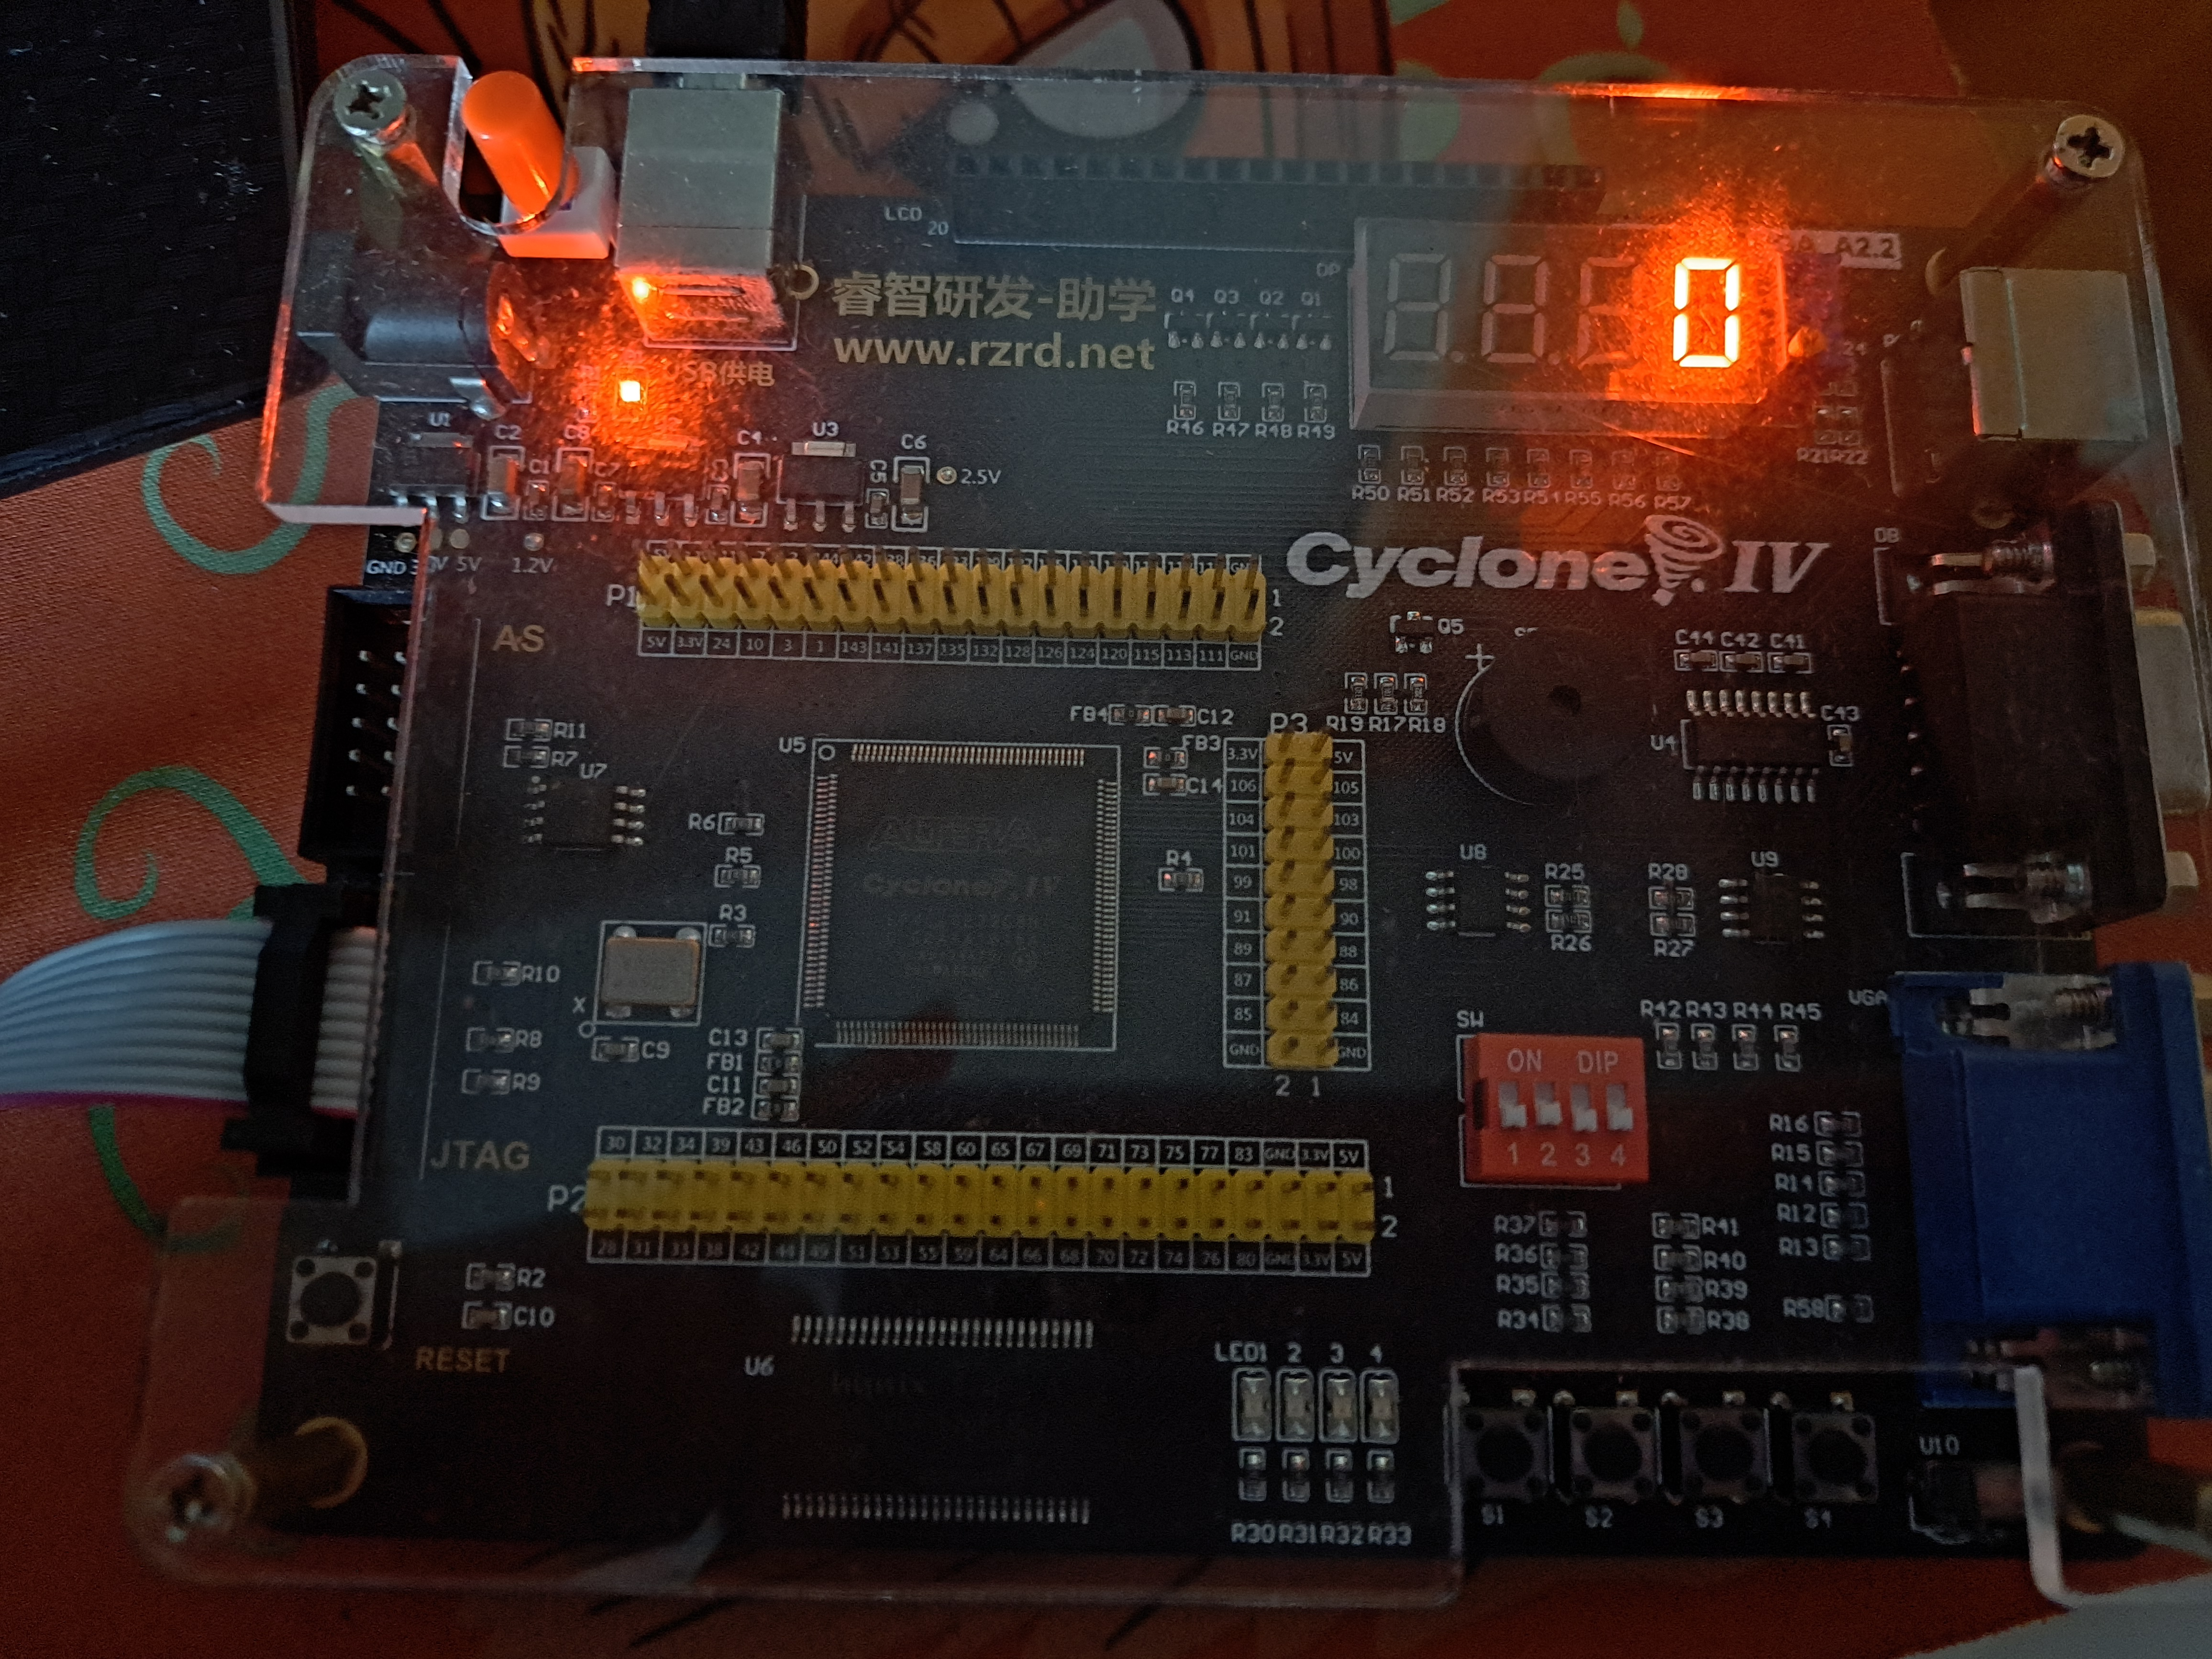
\includegraphics[width=1\columnwidth]{FIGURAS/cap_3/placa0.jpg}
	\caption{Fim do contador decrescente de 10 segundos}
        \label{fig:3.7}
\end{figure}

No total são 16 hexadecimais que precisam ser inseridos e, para cada uma deles, o usuário terá 10 segundos para inseri-los. Toda vez que o usuário errar uma senha, o hardware é reiniciado. Se o usuário inserir o décimo sexto hexadecimal e um buzzer for ativado indefinidamente, isso significa que o usuário acertou todas as 16 senhas. 



\chapter{Resultados}\label{cap_4_Classificacao}

Os requerimentos do projeto foram finalizados. Porém, foram feitas algumas alterações para fins didáticos:

\begin{itemize}
    \item Foi implementado um banco de registradores que armazenam a senha fixa. Esse banco de registradores pode ser visto na seção (2.8).
    \item Os quatro push-buttons foram utilizados para a inserção da senha, com cada um acendendo seu respectivo LED e acionando o buzzer com uma devida frequência. O funcionamento dos push-buttons e dos LED's pode ser visto no manual de operações.
    \item Foi utilizado ambos contadores crescentes e decrescentes. Para aprender o funcionamento de ambos.
    \item Foi implementado, no display de sete segmentos, um contador regressivo para indicar o tempo que o usuário tem para inserir a senha. Esse display pode ser visto no manual de operações.
    \item Foi implementado um contador, que pode funcionar tanto crescente quanto decrescente, de 8 bits, para dividir o clock nas frequências do buzzer, com exceção da frequência de 1Hz. Nela foi utilizado o LPM Counter. Isso pode ser visto na seção 2.4
    \item Foi implementado um debouncer de 110Hz para os push-buttons da placa, que pode ser visto na seção 2.7.
\end{itemize}

\section{Vídeo}

\href{https://drive.google.com/file/d/1tNwCKX1g5BIK9-MFe4KzjO6rrqYe75fk/view?usp=sharing}{Vídeo do funcionamento da placa}

O vídeo acima mostra o funcionamento prático do projeto implementado à placa, a senha armazenada pela placa é "1, 2, 3, 4, 5, 6, 7, 8, 9, 10, 11, 12, 13, 14, 15, 0".

Inicialmente a senha foi inserida corretamente até a entrada do número "3" (três), a quarta entrada foi deixada vazia para que o "0" (zero) seja armazenado, porém como o valor correto é o número "4" (quatro), a placa emite um som grave e reinicia o processo de recebimento da senha.

Nesta nova tentativa, a senha foi inserida corretamente do início ao fim, resultando no sinal audível contínuo do buzzer que só foi interrompido ao desligar a placa.
\chapter{Discussão dos Resultados}\label{cap_5_Resultados}

Neste capitulo será discutido os desafios, e soluções que levaram ao funcionamento do projeto de acordo com as especificações.

\section{O Circuito Completo}

\subsection{Desafios}

O maior desafio encontrado foi o entendimento de processos paralelos. 

Em geral, tinha-se uma tendencia a imaginar que bugs ou inconsistências lógicas do circuito ocorriam pois certas operações estavam fora de ordem.

Para fazer o debug dessa hipótese foi criado uma função buffer de 1bit, para ter-se melhor controle sobre a ordem das operações lógicas na placa. Ela pode ser vista na Figura \ref{fig:5.1}.

\begin{figure}[H]
	\centering
	\includegraphics[width=1\columnwidth]{FIGURAS/cap_5/buffer_1bit.png}
	\caption{Buffer de 1 bit, que foi utilizado para debug.}
        \label{fig:5.1}
\end{figure}

Foi notado que em todos os casos que foi pensado que o bug ocorria por falta de paralelismo, o problema foi erros lógicos da parte do grupo.

Fazer descrição de hardware parece fundamentalmente diferente do que já havia-se visto antes, que foi programação imperativa e sequencial.

\subsection{Soluções}

%Não entendi essa segunda frase
A solução foi uma mudanca da maneira de pensar sobre descrição lógica. Isso para tentar realmente aceitar que os processos de fato ocorrem simultaneamente, e tentar manter lógicas sequenciais restritas a serem atreladas ao clock do FPGA.

\section{Flip-Flops}

\subsection{Desafios}

Não tinha-se costume com a ideia de clear e preset, apresentadas nas Figuras \ref{fig:2.2} e \ref{fig:2.3}.

Houve problemas com como causar um clear ou um preset em um devido flip-flop, sem o "travar" num valor de clear ou preset.

\subsection{Soluções}

Para resolver este problema, foi criado a função pulso, descrita na seção 2.6

Com esta, foi possível transformar um rising\_edge ou falling\_edge do clock como um pulso, que rapidamente ativa o clear ou o preset, e o desliga. Isso foi feito para causar um reset no flip-flop, mas mantê-lo em operação.

\section{Divisores}

\subsection{Desafios}

Foi criado um divisor simples, descrito na figura \ref{fig:2.4}, com lógica decrescente. Isso, devido aos requerimentos do projeto.

Ele funcionou de maneira bem direta. Porém, teve-se problema quando foi tentado o utilizar como contador crescente em cascata com outros Divisor1. Isso foi visto na seção 2.3.2.

O problema é que na primeira subida logica no modo crescente, o $Q$ subiria de 0 para 1. E se esse estiver no input clock do flip-flop seguinte, o seguinte também seria acionado e o $Q$ do seguinte subiria o nivel lógico.

Isso causa um efeito em cascata, no qual a primeira subida do clock inicial do primeiro flip-flop da cascata, acarreta que todos flip-flops são ativados e todos niveis lógicos de todos sobem.

Esse comportamento era indesejado.

\subsection{Soluções}

Com o \emph{Not} na saida do Divisor1, este problema foi resolvido. Isso ocorre já que na primeira subida logica do clock, haverá uma descida lógica da saída, o que não causa ativação do flip-flop seguinte.

\section{Contadores}

\subsection{Desafios}

A dificuldade central com contadores foi fazer o controle do reset e o controle de como o fazer ser crescente ou decrescente.

\subsection{Solucao}

No contador de 8 bits autoral, foi criado uma lógica crescente no contador. Esse contador pode ser feito crescente ou decrescente alterando apenas as suas saídas com um \emph{NOT}.

E com isso foi controlado, não o ponto de parada do contador, mas sim seu \emph{Modulo}. Ou seja. foi possível escolher se começa-se em $255$ ou $0$, e o reset ocorreria quando seu \emph{MOD} for atingido.


\section{Frequências acima de 1Hz}

\subsection{Desafios}

Poderia-se ter utilizado o LPM Counter para fazer a divisão, mas foi resolvido utilizar o contador autoral e divisor de frequência para fins didáticos.

O maior desafio foi definir a precisão que queria-se nas frequências.

\subsection{Soluções}

Pode-se fazer este ser mais preciso utilizando um contador de mais de 8 bits, ou múltiplos contadores de 8 bits.

Por fim resolveu-se escolher o valor que utilize o mínimo de componentes e tenha margem de erro de menos de $1\%$.

Isso permitiu utilizar apenas divisores simples e um contador 8 bits para obter cada frequência.

\section{Pulsos}

\subsection{Desafios}

Ele foi criado para resolver dois problemas. O primeiro foi que precisava-se que componentes fossem ativados tanto na subida de um clock, quanto na descida. O segundo foi o problema do rápido reset/preset de flip-flops.

\subsection{Soluções}

Este pulso resolveu ambos requerimentos e foi utilizado extensivamente no projeto.

\section{Debounce}

\subsection{Desafios}

Teve-se problemas ligando flip-flops diretamente nos push-buttons. 

Crê-se que isso ocorreu pelo botão ser um sistema mecânico e há uma transição imperfeita entre seu estado desligado para seu estado ligado. Isso acarretou que naquela transição, o nível lógico enviado pelo input sobe e desce uma quantidade não previsível de vezes.

\subsection{Soluções}

Foi implementado um debouncer para os botões, Figura \ref{fig:2.14}. Talvez ele funcionaria se utilizasse menos buffers e uma frequência mais alta, Porém, após ele funcionar, não foi tentado otimizá-lo mais.


\section{Registradores}

\subsection{Desafios}

Precisa-se de um sistema que armazene 16 hexadecimais, e faça o ciclo entre eles baseado em um \emph{Rising\_Edge} de entrada.

\subsection{Soluções}

Cria-se o registrador como sugerido, e com este, utiliza-se um contador MOD 16 para controlar a saída de um banco de registradores, alterando o qual registrador será a saída deste banco de registradores, baseado na contagem do contador.

E também usa-se o estouro \emph{Carry\_Out} do contador como o aviso para o sistema que todos hexadecimais foram inseridos corretamente.


\section{Prioridade}

\subsection{Desafios}

Foi encontrado um problema ao apertar um botão enquanto o buzzer estava reproduzindo uma frequência, isso fazia com que houvesse um conflito entre as frequências que foram enviadas ao buzzer. 

\subsection{Soluções}

Para resolver esse problema foi implementado um sistema de prioridades, visto na seção 2.9, que envia para o buzzer a frequência mais recente. Com isso, ao ser enviada alguma frequência, ela irá cancelar todas as outras frequências para enviar a mais recente para o buzzer.

\section{Comparador}

\subsection{Desafios}

Precisa-se de um sistema que realize a comparação entre a entrada do usuário e a senha armazenada nos registradores.

\subsection{Soluções}

Para ser feita a comparação, foi feito um sistema utilizando quatro portas lógicas XOR e uma NOR. Caso os bits nas entradas das portas lógicas XOR forem iguais, a saída delas será 0, portanto, se todas as entradas da porta lógica NOR forem 0 a saída será 1.

\section{LED e Buzzers}

\subsection{Desafios}

Teve-se problemas para conseguir que o buzzer desligue após certo tempo pré-determinado ligado.

\subsection{Soluções}

Utiliza-se o nível lógico do LED para ativar um flip-flop que ativa/desativa um mute switch do buzzer.

E utilizamos também o nível lógico deste mesmo flip-flop para iniciar um divisor de frequências de $2$ Hz que é inserido num contador decrescente MOD 2, como foi requisitado no projeto, isto nos dá uma frequência de saída de $1$ Hz, nesta frequência enviamos um pulso para o reset do flip-flop, para dar mute no buzzer.

\section{Display de sete segmentos}

\subsection{Desafios}

Ao realizar todas as funcionalidades obrigatórias, optamos por desenvolver uma funcionalidade extra ao projeto, que consiste na exibição da saída do contador MOD 10 decrescente no display de sete segmentos.

\subsection{Soluções}

Para isso, ao invés de utilizar apenas o clock de saída do contador MOD 10, monitoramos tambêm as saídas de seus flip-flops com o intuito de exibir em tempo real sua contagem no display de sete segmentos.
\chapter{Conclusão}\label{cap_6_Conclusao}

Pode-se concluir que vários objetivos foram concluídos. O banco de registradores foi implementado. Os quatro push-buttons, seus LED's e suas devidas sonoridas foram implementadas. O contador MOD2 também foi implementado.

%Como limitação, o contador MOD10 autoral não é decrescente como foi requisitado. Ele nesse projeto é crescente, mas com pequenas alterações ele poderia ser crescente.

Houve dificuldades na relação teoria versus prática, pois os push-buttons requeriram um debounce para confirmar que eles estavam, de fato, sendo precionados. O contador MOD10 apresentava erros na FPGA quando havia sua mudança para ser decrescente.

A realização do relatório foi muito importante para o grupo. Isso porque, foi pela realização dele, que foi possível ter discussões sobre como melhorar o projeto e sobre o que cada arquivo do quartus fazia. Também foi possível, para cada integrante do grupo, compreender melhor todas as partes do projeto, já que a elaboração do relatório incentivou o diálogo entre todos os integrantes do grupo e, consequentemente, levou a um melhor trabalho na equipe.




%\chapter[TÍTULO CURTO PARA APARECER NO SUMÁRIO(CASO NECESSÁRIO)]{TÍTULO DO CAPÍTULO, TEM QUE SER ESCRITO EM MAIÚSCULO}
\label{cap_Exemplo}

Toda equação deve ser citada no texto, A Eq. (\ref{eq:5.1}) exemplifica uma equação. Use o editor de equações no seguinte link \url{https://latex.codecogs.com/eqneditor/editor.php}

\begin{equation}\label{eq:5.1}
\mathbf{F}=\mathbf{E}\mathbf{\Lambda}\mathbf{E}^T,
\end{equation}

Exemplo de tabela:

\begin{table}[htb]
\ABNTEXfontereduzida
\caption[Multiplicidade dos autovalores da matriz $N \times N$ da DFT.]{Multiplicidade dos autovalores da matriz $N \times N$ da DFT.}
\label{tab:eigenval_real}
\begin{center}
	\begin{tabular}{c|cccc}
          \hline
            $N$  &  $1$    &  $-i$   &  $-1$ &  $i$  \\ \hline
        $4L$  & $L+1$ & $L  $ & $L$ & $L-1  $  \\ [3pt]
        $4L+1$& $L+1$ & $L  $ & $L  $ & $L  $  \\ [3pt]
        $4L+2$& $L+1$ & $L$ & $L+1  $ & $L  $ \\ [3pt]
        $4L+3$& $L+1$ & $L+1$ & $L+1  $ & $L$\\ [3pt]
          \hline
        \end{tabular}
\end{center}       
\legend{Fonte:~\cite{McClellan}.}
\end{table}

\section{SEÇÃO TAMBÉM ESCRITO EM MAIÚSCULO}\label{sec:related}

Exemplo de teorema:

\begin{theorem}\label{theo:optimal} \cite{Kuznetsov_2015}~
Assumindo que $N\geq 3$,
\vspace{-0.5cm}
\begin{enumerate}
\item[i.] Se $N = 2K +1$, existem apenas $K+1$ vetores pares não-nulos que satisfazem $l(\mathbf{u})+l(\mathbf{Fu}) = N +1$ e apenas $K$ vetores ímpares não-nulos satisfazendo $l(\mathbf{v}) + l(\mathbf{Fv}) \leq N + 3$.
\item[ii.] Se $N = 2K$, existem apenas $K - 1$ vetores pares não-nulos que satisfazem $u(K) = (Fu)(K)= 0$ e
$l(\mathbf{u}) + l(\mathbf{Fu}) \leq N + 2$ e apenas $K - 1$ vetores ímpares  não-nulos satisfazendo $l(\mathbf{v}) + l(\mathbf{Fv}) \leq N + 2$.
\end{enumerate}
\end{theorem}
Em~\cite{Kuznetsov_2015}, expressões explícitas para os vetores descritos no Teorema~~\ref{theo:optimal} são dadas para todos os valores de $N$. A seguir, descreve-se como construir esses vetores para $N=4L+1$.


\subsection{Subseção escrito em minúsculo}\label{sec:pei}

Exemplo de figura:

\begin{figure}[!hpt] 
	\centering	
	\caption[Distribuição dos autovalores de $\mathbf{S}_{\overline{\mathbf{T}}}$ no plano complexo.]{Distribuição dos autovalores de $\mathbf{S}_{\overline{\mathbf{T}}}$ no plano complexo, para~\subref{imaeig} $N=5$,~\subref{imbeig} $N=9$,~\subref{imceig} $N=13$ e~\subref{imdeig} $N=17$.}
	\label{fig:eigs}
\subfloat[][]{\label{imaeig}\includegraphics[scale=0.31]{./FIGURAS/cap_Exemplo/eigenvaluesn.pdf}}\hspace{0.05cm}
\subfloat[][]{\label{imbeig}\includegraphics[scale=0.31]{./FIGURAS/cap_Exemplo/eigenvalues1n.pdf}}\hspace{0.05cm}
\subfloat[][]{\label{imceig}\includegraphics[scale=0.31]{./FIGURAS/cap_Exemplo/eigenvalues2n.pdf}}\hspace{0.05cm}
\subfloat[][]{\label{imdeig}\includegraphics[scale=0.31]{./FIGURAS/cap_Exemplo/eigenvalues3n.pdf}}
\legend{Fonte:~\cite{Neto_2017}.}
\end{figure}






% ----------------------------------------------------------
% ELEMENTOS PÓS-TEXTUAIS
% ----------------------------------------------------------
\begin{comment}
    

\postextual
% ----------------------------------------------------------

% ----------------------------------------------------------
% Referências bibliográficas
% ----------------------------------------------------------
%\bibliography{abntex2-modelo-references}
\bibliography{bib_tese}{}
\markboth{REFERÊNCIAS}{ }


% ----------------------------------------------------------
% Glossário
% ----------------------------------------------------------
%
% Consulte o manual da classe abntex2 para orientações sobre o glossário.
%
%\glossary

% ----------------------------------------------------------
% Apêndices
% ----------------------------------------------------------

% ---
% Inicia os apêndices
% ---
\begin{apendicesenv}

%\chapter[]{TÍTULO DO APÊNDICE}
%\addcontentsline{toc}{chapter}{AP\^ENDICE}
\markboth{AP\^ENDICE}{ }
\label{apendice:A}

Elemento opcional. Texto ou documento não elaborado pelo autor, que serve de fundamentação, comprovação e ilustração.


\end{apendicesenv}
% ---


% ----------------------------------------------------------
% Anexos
% ----------------------------------------------------------

% ---
% Inicia os anexos
% ---
%\begin{anexosenv}
%
%% Imprime uma página indicando o início dos anexos
%%\partanexos
%
%\chapter*{ANEXO}
%\label{ch:anexo}
%\addcontentsline{toc}{chapter}{ANEXO}
%\markboth{ANEXO}{ANEXO}
%
%\begin{center}
%IMAGENS DE TESTE UTILIZADAS
%\end{center}
%
%\lipsum[1]
%
%
%\end{anexosenv}

%---------------------------------------------------------------------
% INDICE REMISSIVO
%---------------------------------------------------------------------
\phantompart
\printindex
%---------------------------------------------------------------------
\end{comment}
\end{document}
